\section{Positioning solutions}\label{sec:sprint1-pozyx}
Since positioning is a major part of the project, it is important to have accurate positioning information.
A positional system named Pozyx was supplied for this semester, and will be used for generating position data.
Along with Pozyx, this section will describe some alternatives in order to examine if any can be used to supplement the Pozyx system.
Pozyx is a hardware/software solution that is used to provide positioning with an accuracy of down to 10 cm \cite{pozyx}.
It makes use of ultra-wide band (UWB) in combination with machine learning for positioning \cite{pozyx}, which according to their documentation is more precise and efficient than traditional positioning systems such as WiFi, Bluetooth, RFID, and GPS.
\\\\
Pozyx consists of sensors called anchors and tags.
Anchors are stationary sensors which the moveable tags use to measure their position, based on how far away these tags are. 
The anchors define the dimensions of the playing field and the players and the ball are equipped with the tags to allow their positions to be found.

\subsection{Finding the location of anchors}
A trilateration method is used for finding the position of a given tag using the anchors.
This method uses basic geometry to estimate the position by measuring the distance to the anchors of which we know the position.
With this distance estimate, it is possible to draw a circle with a given radius.
If we use two anchors, we will have two intersection points which are the possible positions of the tag.
This means that to find a two-dimensional location, we will need at least three anchors, which will lead to only a single point where all three circles intersect, as seen on \autoref{fig:trilateration}.

\begin{figure}[H]
    \centering
    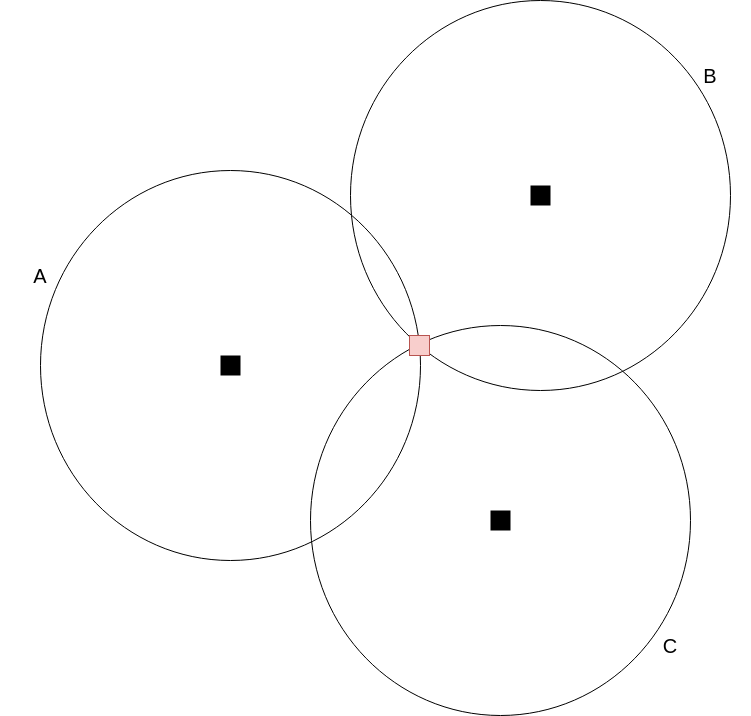
\includegraphics[width=0.6\linewidth]{trilateration.png}
    \caption{An example of trilateration using three anchors.}
    \label{fig:trilateration}
\end{figure}

\noindent
The issue with this approach is that the measurements are not perfect, which might cause the circles to not intersect at exactly one point which will make the positional data seem to jitter.

\subsection{Using UWB}
To find the distance between a tag and the anchors, Pozyx makes use of radio waves.
Radio waves travel at the speed of light \cite{pozyx-UWB}, so by dividing the time of travel between anchors with the speed of light, the distance between them can be found.\\
Because the speed of light is so fast the time measure needs to be very accurate to get the correct distance.
To achieve this the anchors make use of UWB \cite{pozyx-UWB}.
UWB is a technology for transmitting data over a wide bandwidth usually wider than 500 MHz.
The Pozyx sensors use exactly 500 MHz which means they just qualify as a UWB system.
Because the bandwidth is this wide it makes the wavelength very short, and by combining multiple sinusoidal signals with slightly different frequencies the Pozyx tags can create a pulse with a peak which is very narrow.
Measuring a narrow peak results in a more accurate timing, allowing the Pozyx to be much more precise than other technologies like Bluetooth and WiFi.
High bandwidth means faster data transfer, which most people would prefer, but if everyone were to use the same frequency the signals would interfere with each other, therefore the use of high-frequency signals is tightly regulated \cite{tait-radio}.
To reduce the amount of interference the regulations say that UWB systems may only transmit at very low power.
This means that a UWB transmission can not travel very far and therefore the chance of it interfering with another system is very low.
Because of this we are not able to build huge playing fields with the limited amount of anchors we have if we also want it to be precise or even playable.
Building a playing field that is larger than the anchors can reach could cause some tags to not reach all anchors and therefore not calculate a position.
This could be combated somewhat by having more anchors, but as will be explained in \ref{pozyx:TWR} this is not a viable solution.


\subsection{Two-way-ranging} \label{pozyx:TWR}
We are using the Pozyx Creator Kit Lite package, which uses the Two-way-ranging (TWR) protocol for positioning \cite{pozyx-Positioning}.\\
A tag calculates its position by communicating with the anchors one by one, getting the distance from the anchor to itself.
Once it has the distance from 3 anchors it can compute its position utilizing trilateration.
\\
If multiple tags are being used at once, one tag is made the master tag and the other tags become the slave tags.
The master tag instructs the slave tags to report their position to the master tag one by one.
The master tag is then usually connected to a computer that can use the position data.
This technique does not scale well as all the slave tags have to be within the radio range of the master tag so spreading them across huge areas is not possible.
Instead of a tag being the master it is possible to use an anchor.\\
This makes it easier to have a computer attached, as the anchors are stationary, unlike the tags.

\subsection{Alternatives to UWB}
Having a high accuracy is essential for the users' experience since a low accuracy could result in the in-game information being incorrect or just too imprecise to make it a joyful experience.
While Pozyx uses UWB for positioning, it is interesting to take a look at the primary alternatives to indoor positioning and to see if any of them can compete with Pozyx' high accuracy \cite{pozyx}, or be used in combination with it.

\subsubsection{GPS}
The obvious alternative for positioning data is GPS, which is frequently used for outdoor positioning.
In optimal outdoor situations, GPS can provide accuracy within 4.9 meters \cite{gpsgov:accuracy}.
However, the GPS positioning accuracy can be degraded due to buildings, bridges, and trees, making it a sub-optimal choice for indoor positioning.

\subsubsection{Wi-Fi}
Since the project will most likely utilize networking for data transfer, Wi-Fi may be worth considering to decrease the number of technologies needed.
However, Wi-Fi only provides an accuracy of between 5 and 15 meters depending on the hardware chosen for access points and clients.\\
In addition to this, iOS devices are blocked from using Wi-Fi for indoor navigation purposes, since it usually makes use of a technology called fingerprinting, which only functions with Android devices due to technical restrictions \cite{infsoft:wifi}.

\subsubsection{Bluetooth}
Using Bluetooth for indoor location is similar to how Pozyx works with anchors and tags.
Instead of anchors, Bluetooth beacons are able to send out signals with a range of up to 30 meters \cite{infsoft:bluetooth}.
With Bluetooth, you get a significantly higher accuracy compared to GPS and Wi-Fi.
In the optimal settings, this solution can provide an accuracy of up to one meter.
Unlike Wi-Fi, this solution would work on both iOS and Android devices.

\subsubsection{RFID}
Finally, we have RFID which uses radio waves to wirelessly transmit the identity of an object.
Unlike the other solutions, RFID offers high accuracy, but a very limited range of less than a meter \cite{infsoft:rfid}.\\
For a game like the one in this project, it would be possible to use RFID for the location of the ball to check which player is currently holding it, but due to the limited range, it would not make sense to use it for localizing the players.\\
